% Apêndice A - Fluxogramas baseados nos microflows da aplicação
% Requer \usepackage{pdflscape} e \usetikzlibrary{shapes.geometric,calc,fit} no preâmbulo.

\begin{apendicesenv}
\chapter{Lógica de salvamento de uma ocorrência}
\label{ap:salvar}

Este apêndice apresenta a lógica executada quando o usuário salva a descrição do problema de uma nova ocorrência, modelada no Mendix em \textit{microflows} (Seção~\ref{sec:mendix}). Em vez de capturas de tela, optou-se por fluxogramas elaborados pelo autor, por dois motivos: os originais trazem nomes em inglês e detalhes de implementação que dificultariam a leitura, e seus nomes de módulos e entidades permitiriam identificar a organização. Os fluxogramas mantêm a sequência de atividades e decisões, com nomes traduzidos e generalizados.

Antes de gravar o registro, a aplicação valida os campos obrigatórios da descrição do problema, em cinco grupos de verificação, como mostra a Figura~\ref{fig:mf-validar}. Basta um campo pendente para que a ocorrência não seja salva, e a mensagem aparece junto ao campo correspondente.

Concluída a validação, o fluxo principal (Figura~\ref{fig:mf-salvar}) gera o identificador da ocorrência ou, se ela era um rascunho, muda sua situação para aberta. Em seguida, envia o registro ao sistema de controle de \textit{tickets}, que devolve o número do chamado, avança a ocorrência para a ação de contenção, carrega a configuração de verificação da unidade, registra o histórico, vincula os anexos e salva a ocorrência. Por fim, aciona a sirene e dispara as notificações. Se a validação ou a integração falharem, nada é salvo, e por isso não existe ocorrência sem um chamado vinculado.

\begin{figure}[htbp]
    \centering
    \caption{Fluxograma baseado no \textit{microflow} de validação da descrição do problema}
    \label{fig:mf-validar}
    \resizebox{\textwidth}{!}{%
    \begin{tikzpicture}[fx, fxproc/.append style={text width=3.0cm, minimum width=3.3cm}]
    \simbolosFX{-4.4,0.4}{fxtermleg/Terminal, fxdecleg/Decisão, fxprocleg/Processamento, fxconleg/Conector}{4}
    % ---------- coluna 1
    \node[fxterm] (ini) at (0,0) {Início};
    \node[fxproc, below=of ini] (v1) {Verificar tipo e descrição: tipo preenchido e descrição do problema preenchida};
    \node[fxdec, below=of v1] (d1) {Tipo e descrição OK?};
    \node[fxproc, below=of d1] (v2) {Verificar local e responsável pela detecção: no tipo segurança, formulário de segurança; nos demais, detectado por, turno, cliente, linha, produto e revisão e sintoma};
    \node[fxdec, below=of v2] (d2) {Detecção OK?};
    \node[fxcon, below=of d2] (c1) {1};
    \node[fxcon] (e1) at ($(d1)+(2.5,0)$) {2};
    \node[fxcon] (e2) at ($(d2)+(2.5,0)$) {2};
    % ---------- coluna 2
    \node[fxcon] (c1b) at (5.4,0) {1};
    \node[fxproc, below=of c1b] (v3) {Verificar a dimensão do problema: frequência e quantidade preenchidas};
    \node[fxdec, below=of v3] (d3) {Dimensão OK?};
    \node[fxproc, below=of d3] (v4) {Verificar a categoria: ao menos uma assinalada; se ``outros'', descrição obrigatória};
    \node[fxdec, below=of v4] (d4) {Categoria OK?};
    \node[fxcon, below=of d4] (c2) {3};
    \node[fxcon] (e3) at ($(d3)+(2.5,0)$) {2};
    \node[fxcon] (e4) at ($(d4)+(2.5,0)$) {2};
    % ---------- coluna 3
    \node[fxcon] (c2b) at (10.8,0) {3};
    \node[fxproc, below=of c2b] (v5) {Verificar os cadastros: cliente e unidade existentes};
    \node[fxdec, below=of v5] (d5) {Cadastros OK?};
    \node[fxterm, below=of d5] (ok) {Fim: descrição válida};
    \node[fxcon] (e5) at ($(d5)+(2.5,0)$) {2};
    \node[fxcon, below=of ok] (eb) {2};
    \node[fxterm, below=of eb] (erro) {Fim: mensagem junto ao campo pendente; nada é salvo};
    \foreach \a/\b in {ini/v1, v1/d1, v2/d2, c1b/v3, v3/d3, v4/d4, c2b/v5, v5/d5, eb/erro} { \draw[fxseta] (\a) -- (\b); }
    \foreach \a/\b in {d1/v2, d2/c1, d3/v4, d4/c2, d5/ok} { \draw[fxseta] (\a) -- node[fxrot, left, pos=0.4]{Sim} (\b); }
    \foreach \a/\b in {d1/e1, d2/e2, d3/e3, d4/e4, d5/e5} { \draw[fxseta] (\a) -- node[fxrot, above, pos=0.4]{Não} (\b); }
    \node[fxquadro, fit=(current bounding box)] {};
    \end{tikzpicture}}
    \legend{Fonte: elaborado pelo autor (2026), com base no \textit{microflow} de validação da aplicação, no Mendix Studio Pro.}
\end{figure}

\begin{landscape}
\begin{figure}[p]
    \centering
    \caption{Fluxograma baseado no \textit{microflow} de salvamento de uma ocorrência}
    \label{fig:mf-salvar}
    \resizebox{\linewidth}{!}{%
    \begin{tikzpicture}[fx]
    \simbolosFX{-4.3,0.4}{fxtermleg/Terminal, fxdecleg/Decisão, fxprocleg/Processamento, fxsubleg/Subprocesso, fxconleg/Conector}{5}
    % ---------- coluna 1
    \node[fxterm] (ini) at (0,0) {Início};
    \node[fxsub, below=of ini] (val) {Validar a descrição do problema (Figura~\ref{fig:mf-validar})};
    \node[fxdec, below=of val] (ok) {Campos válidos?};
    \node[fxfim, text width=1.6cm, minimum width=1.8cm] (f1) at ($(ok)+(3.1,0)$) {Fim: nada é salvo};
    \node[fxdec, below=of ok] (rasc) {Era um rascunho?};
    \node[fxproc, below=of rasc] (id) {Gerar o identificador da ocorrência};
    \node[fxproc] (aberta) at ($(id)+(3.4,0)$) {Mudar a situação para aberta};
    \node[fxcon, below=0.9cm of id] (c1) {1};
    \coordinate[below=0.4cm of id] (m1);
    \draw[fxseta] (ini) -- (val);
    \draw[fxseta] (val) -- (ok);
    \draw[fxseta] (ok) -- node[fxrot, above, pos=0.4]{Não} (f1);
    \draw[fxseta] (ok) -- node[fxrot, left, pos=0.4]{Sim} (rasc);
    \draw[fxseta] (rasc) -- node[fxrot, left, pos=0.4]{Não} (id);
    \draw[fxseta] (rasc.east) -- node[fxrot, above, pos=0.3]{Sim} (rasc.east -| aberta) -- (aberta);
    \draw (id) -- (m1);
    \draw (aberta.south) |- (m1);
    \draw[fxseta] (m1) -- (c1);
    % ---------- coluna 2
    \node[fxcon] (c1b) at (7.3,0) {1};
    \node[fxproc, below=of c1b] (desc) {Gerar a descrição resumida};
    \node[fxsub, below=of desc] (post) {Enviar ao sistema de \textit{tickets} e receber o número do chamado};
    \node[fxdec, below=of post] (suc) {Chamado criado?};
    \node[fxcon] (c2) at ($(suc)+(2.4,0)$) {2};
    \node[fxproc, below=of suc] (log) {Registrar o erro};
    \node[fxfim, below=of log] (f2) {Fim};
    \foreach \a/\b in {c1b/desc, desc/post, post/suc, log/f2} { \draw[fxseta] (\a) -- (\b); }
    \draw[fxseta] (suc) -- node[fxrot, above, pos=0.4]{Sim} (c2);
    \draw[fxseta] (suc) -- node[fxrot, left, pos=0.4]{Não} (log);
    % ---------- coluna 3
    \node[fxcon] (c2b) at (11.9,0) {2};
    \node[fxproc, below=of c2b] (cont) {Avançar para a ação de contenção};
    \node[fxproc, below=of cont] (conf) {Carregar a configuração de verificação da unidade};
    \node[fxproc, below=of conf] (hist) {Registrar o histórico e a configuração da ocorrência};
    \node[fxproc, below=of hist] (anexo) {Vincular os anexos à ocorrência};
    \node[fxcon, below=of anexo] (c3) {3};
    \foreach \a/\b in {c2b/cont, cont/conf, conf/hist, hist/anexo, anexo/c3} { \draw[fxseta] (\a) -- (\b); }
    % ---------- coluna 4
    \node[fxcon] (c3b) at (15.6,0) {3};
    \node[fxdec, below=of c3b] (temid) {Identificador gerado?};
    \node[fxfim] (f3) at ($(temid)+(2.5,0)$) {Fim};
    \node[fxproc, below=of temid] (salva) {Salvar a ocorrência};
    \node[fxproc, below=of salva] (msg) {Exibir a confirmação ao usuário};
    \node[fxcon, below=of msg] (c4) {4};
    \draw[fxseta] (c3b) -- (temid);
    \draw[fxseta] (temid) -- node[fxrot, above, pos=0.4]{Não} (f3);
    \draw[fxseta] (temid) -- node[fxrot, left, pos=0.4]{Sim} (salva);
    \foreach \a/\b in {salva/msg, msg/c4} { \draw[fxseta] (\a) -- (\b); }
    % ---------- coluna 5
    \node[fxcon] (c4b) at (21.2,0) {4};
    \node[fxproc, below=of c4b] (sir) {Acionar a sirene};
    \node[fxsub, below=of sir] (not) {Enviar notificações: e-mail aos envolvidos e alerta aos painéis};
    \node[fxterm, below=of not] (fim) {Fim};
    \foreach \a/\b in {c4b/sir, sir/not, not/fim} { \draw[fxseta] (\a) -- (\b); }
    \node[fxquadro, fit=(current bounding box)] {};
    \end{tikzpicture}}
    \legend{Fonte: elaborado pelo autor (2026), com base no \textit{microflow} de salvamento da aplicação, no Mendix Studio Pro.}
\end{figure}
\end{landscape}

\chapter{Esquema elétrico de acionamento da sirene}\label{ap:sirene}

A Figura~\ref{fig:esquema-sirene} apresenta o esquema elétrico usado para acionar a sirene a partir da aplicação, integração descrita na Seção~\ref{subsec:integracoes}. A parte superior da figura mostra a pinagem do Raspberry Pi, com o GPIO22 destacado em verde, e a parte inferior mostra a ligação entre os componentes. Quando uma ocorrência é criada, ou quando o botão de sirene do painel é acionado, a aplicação envia um comando por API REST ao Raspberry Pi instalado na área produtiva. O Raspberry Pi coloca em nível alto a saída GPIO22 (pino físico 15), que é o pino padrão do acionamento e não pode ser alterado. Essa saída comanda a entrada do módulo de relé, alimentado pelos pinos de alimentação (VCC) e terra (GND) do próprio Raspberry Pi.

Com o relé energizado, o contato comum (C) fecha com o contato normalmente aberto (NA) e a fonte de alimentação passa a alimentar a sirene; quando a saída volta a nível baixo, o contato abre e a sirene desliga. O relé separa o circuito lógico do Raspberry Pi, de baixa corrente, do circuito de potência da sirene, que tem alimentação própria. Assim, a corrente da sirene não circula pela saída do Raspberry Pi, que apenas comanda o relé. O esquema apresenta apenas a lógica de ligação, para delimitar o escopo da solução: as tensões, as correntes e os modelos dos componentes foram omitidos propositalmente, pois dependem da sirene e da fonte adotadas em cada instalação. Para a implementação, devem ser consultados os manuais dos componentes escolhidos e verificada a compatibilidade entre eles. A sinaleira, também acionada a cada ocorrência criada (Seção~\ref{subsec:integracoes}), é ligada ao mesmo relé e, por isso, é acionada junto com a sirene; ela não foi representada separadamente no esquema.

\begin{figure}[htbp]
    \centering
    \caption{Esquema elétrico de acionamento da sirene}\label{fig:esquema-sirene}
    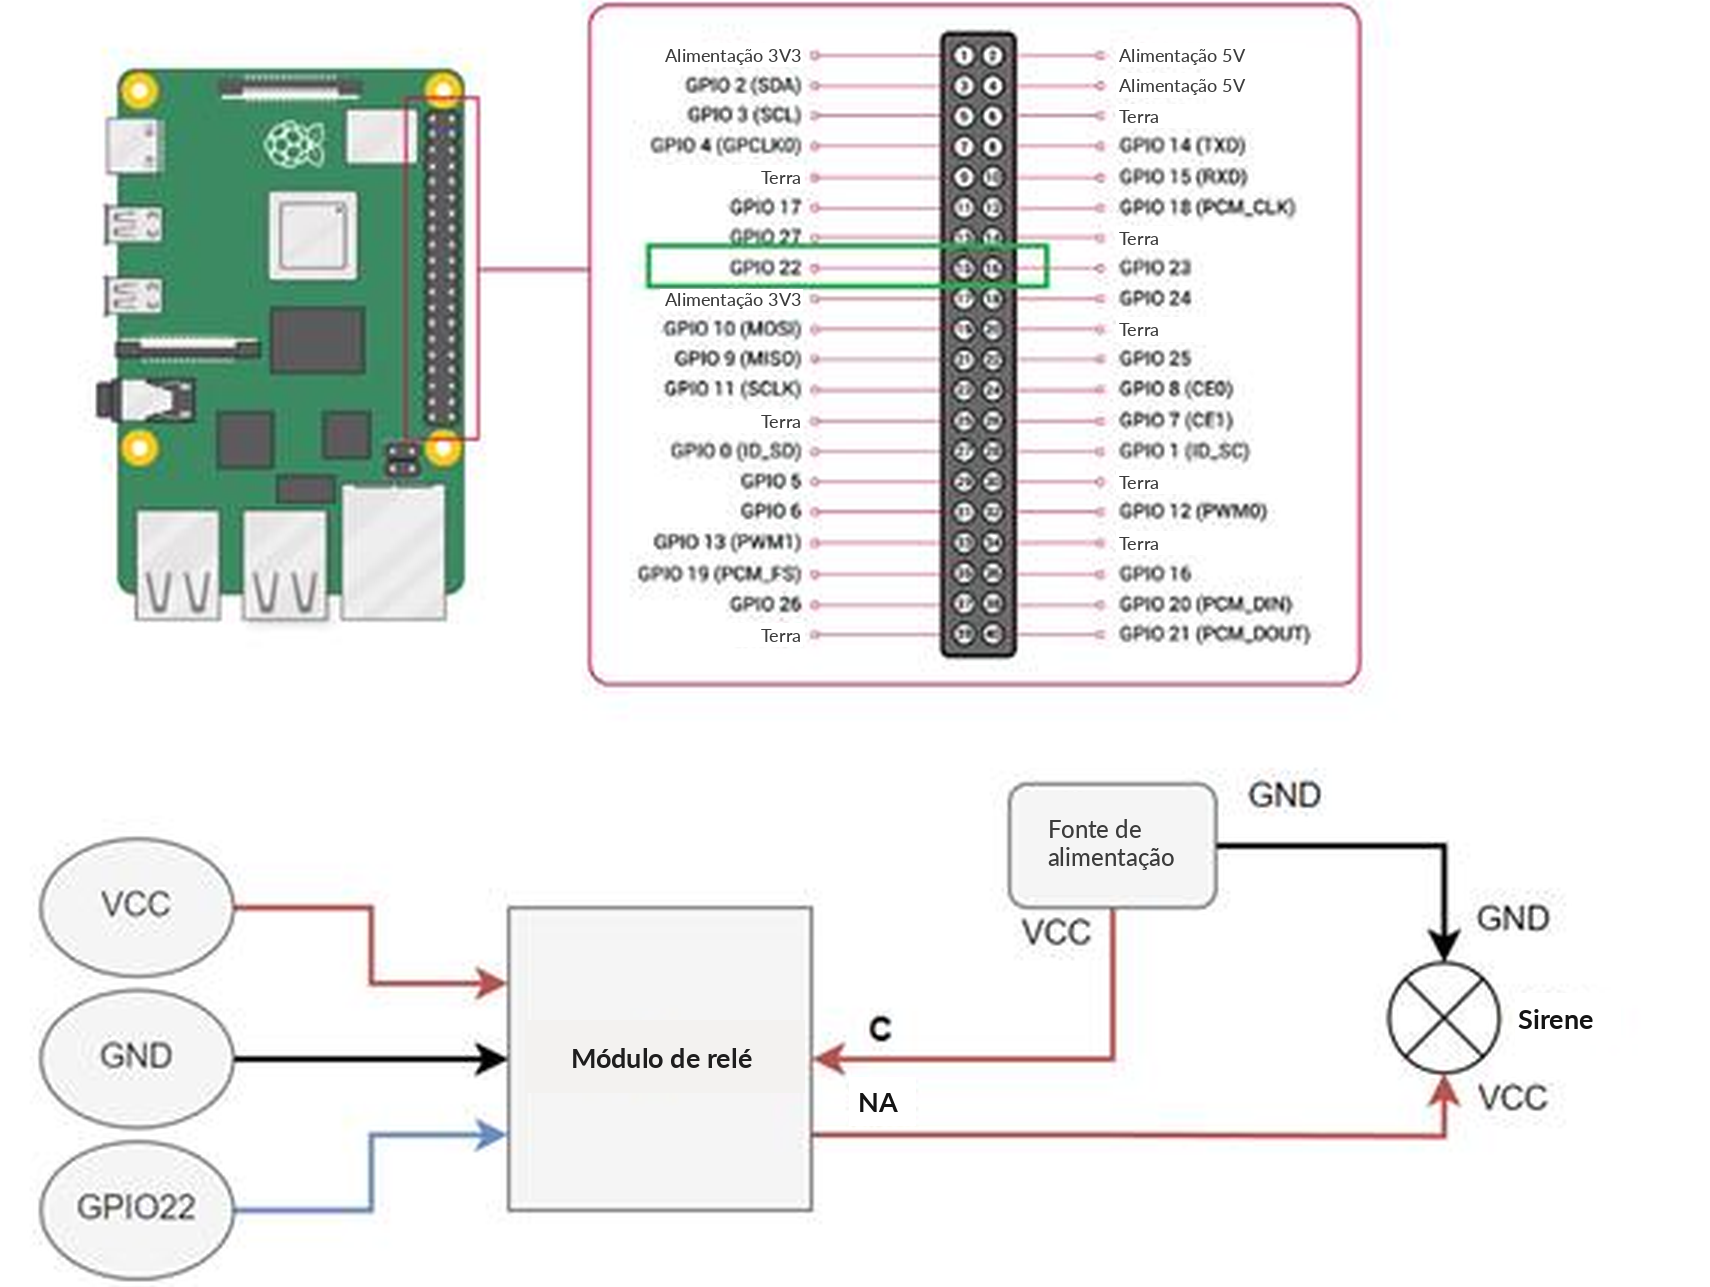
\includegraphics[width=0.95\textwidth]{Figuras/esquema-sirene.png}
    \legend{Fonte: documentação interna da aplicação, traduzido pelo autor (2026).}
\end{figure}
\end{apendicesenv}
